\section{HỆ BẤT PHƯƠNG TRÌNH BẬC NHẤT HAI ẨN}

\subsection{TÓM TẮT LÝ THUYẾT}
\subsubsection{Hệ bất phương trình bậc nhất hai ẩn}
\begin{itemize}
	\item [\iconMT] Là hệ bất phương trình gồm hai hay nhiều bất phương trình bậc nhất hai ẩn.
	\item [\iconMT] Cặp số $(x_0;y_0)$ là nghiệm của hệ bất phương trình bậc nhất hai ẩn khi $(x_0;y_0)$ đồng thời là nghiệm của tất cả các bất phương trình trong hệ đó.
\end{itemize}
\subsubsection{Biểu diễn miền nghiệm của hệ bất phương trình bậc nhất hai ẩn}
\begin{itemize}
	\item [\iconMT] Miền nghiệm của hệ là giao các miền nghiệm của các bất phương trình trong hệ.
	\item [\iconMT] Để biểu diễn miền nghiệm của hệ, ta làm như sau:
	\begin{boxdn}
	\begin{itemize}
		\item [$\bullet$] Trên cùng một mặt phẳng tọa độ, xác định miền nghiệm của mỗi bất phương trình bậc nhất hai ẩn trong hệ và gạch bỏ miền còn lại.
		\item [$\bullet$] Miền cuối cùng không bị gạch là miền nghiệm của hệ bất phương trình đã cho.
	\end{itemize}
	\end{boxdn}
\end{itemize}
\begin{vidu}
Biểu diễn hình học tập nghiệm của hệ bất phương trình
$\heva{& 3x+y\leq 6 \quad (1)\\& x+y\leq 4 \quad(2)\\& x\geq 0 \quad(3)\\& y\geq 0 \quad(4).} \quad(\star)$, ta làm như sau: 
	\begin{itemize}
		\item [$\bullet$] Vẽ đường thẳng $d_1 \colon 3x+y=6$.\\
		Lấy điểm $M(1;1)$, thay tọa độ $M$ vào bất phương trình (1), ta được $3 \cdot 1 + 1 \le 6$ (thỏa mãn). Suy ra miền nghiệm của bất phương trình (1) là phần không bị gạch như hình vẽ 1, kể cả những điểm nằm trên $d_1$.
		\item [$\bullet$] Tương tự cho bất phương trình (2) (Hình 2) và bất phương trình (3) và (4) (Hình 3).
		\begin{tikzpicture}[line join=round, line cap=round, >=stealth,font=\footnotesize, scale=0.6]
			\draw[->](-2,0)--(3,0) node[below right] {$x$};
			\draw[->](0,-1)--(0,5) node[above] {$y$};
			\node (0,0) [below left]{$ O $};
			\foreach \x in {-1,...,2}
			\draw[shift={(\x,0)},color=black] (0pt,2pt) -- (0pt,-2pt);
			\foreach \y in {1,...,5}
			\draw[shift={(0,\y)},color=black] (2pt,0pt) -- (-2pt,0pt);
			\draw[samples=100,smooth,domain=0.333:2.333] plot(\x,{-3*(\x)+6});
			\fill[pattern=north west lines,pattern color=orange] (0.333,5)--(3,5)--(3,-1)--(2.333,-1)--cycle;
			\draw[dashed] (1,0)node[below] {$1$}--(1,1)node[above] {$M$}--(0,1)node[left] {$1$};
			\node[below] at (0,-1.4) {Hình 1};
			\end{tikzpicture}
		\hspace{1.4cm}
		\begin{tikzpicture}[line join=round, line cap=round, >=stealth,font=\footnotesize, scale=0.6]
			\draw[->](-2,0)--(3,0) node[below right] {$x$};
			\draw[->](0,-1)--(0,5) node[above] {$y$};
			\node (0,0) [below left]{$ O $};
			\foreach \x in {-1,...,2}
			\draw[shift={(\x,0)},color=black] (0pt,2pt) -- (0pt,-2pt);
			\foreach \y in {1,...,5}
			\draw[shift={(0,\y)},color=black] (2pt,0pt) -- (-2pt,0pt);
			\draw[samples=100,smooth,domain=0.333:2.333] plot(\x,{-3*(\x)+6});
			\draw[samples=100,smooth,domain=-1:3] plot(\x,{-(\x)+4});
			\fill[pattern=north west lines,pattern color=orange] (0.333,5)--(3,5)--(3,-1)--(2.333,-1)--cycle;
			\fill[pattern=crosshatch dots,pattern color=blue] (-1,5)--(3,5)--(3,1)--cycle;
			\node[below] at (0,-1.4) {Hình 2};
		\end{tikzpicture}
	\hspace{1.4cm}
	\begin{tikzpicture}[line join=round, line cap=round, >=stealth,font=\footnotesize, scale=0.6]
		\draw[->](-2,0)--(3,0) node[below right] {$x$};
		\draw[->](0,-1)--(0,5) node[above] {$y$};
		\node (0,0) [below left]{$ O $};
		\foreach \x in {-1,...,2}
		\draw[shift={(\x,0)},color=black] (0pt,2pt) -- (0pt,-2pt);
		\foreach \y in {1,...,3}
		\draw[shift={(0,\y)},color=black] (2pt,0pt) -- (-2pt,0pt);
		\draw[samples=100,smooth,domain=0.333:2.333] plot(\x,{-3*(\x)+6});
		\draw[samples=100,smooth,domain=-1:3] plot(\x,{-(\x)+4});
		\fill[pattern=north west lines,pattern color=orange] (0.333,5)--(3,5)--(3,-1)--(2.333,-1)--cycle;
		\fill[pattern=crosshatch dots,pattern color=blue] (-1,5)--(3,5)--(3,1)--cycle;
		\fill[pattern=north east lines,pattern color=cyan] (-2,-1)--(-2,5)--(0,5)--(0,-1)--cycle;
		\fill[pattern=crosshatch dots,pattern color=magenta] (-2,-1)--(-2,0)--(3,0)--(3,-1)--cycle;
		\node[below] at (0,-1.4) {Hình 3};
	\end{tikzpicture}
		\item [$\bullet$] Miền không bị tô đậm (hình tứ giác kể cả bốn cạnh của nó) trong hình vẽ bên là miền nghiệm của hệ bất phương trình đã cho.
	\end{itemize}
\end{vidu}
\subsection{RÈN LUYỆN KĨ NĂNG GIẢI TOÁN}
\begin{dang}{Nghiệm của hệ bất phương trình bậc nhất hai ẩn.}
\end{dang}

\begin{vd}
	Cho hệ bất phương trình bậc nhất hai ẩn $\heva{&x+y>0\\&x+2y<9}$. Tìm tất cả các cặp số $(x_0;y_0)$ có tọa độ nguyên là nghiệm của hệ đã cho, biết $x_0=-1$.
	\loigiai{
	Thay $x=1$ và hệ, ta được $\heva{&-1+y>0\\&-1+2y<9} \Leftrightarrow 1<y<5$.\\
	 Chọn $y \in \{2;3;4\}$, ta được các cặp nghiệm là $(1;2)$, $(1;3)$, $(1;4)$.}
\end{vd}

\begin{vd}
	\immini{Cho hệ bất phương trình bậc nhất hai ẩn $\heva{& 3x+y\leq 6 \\& x+y\leq 4 \\& x\geq 0 \\& y\geq 0 .}$ có miền nghiệm là phần không bị gạch như hình bên (tứ giác $OABC$, bao gồm các cạnh). 
		\begin{tasks}(1)
			\task Tìm những cặp nghiệm có tọa độ nguyên của hệ bất phương trình trên.
			\task Xác định tọa độ 3 đỉnh $A$, $B$ và $C$. Tính diện tích tứ giác $OABC$.
		\end{tasks}
		
	}{
	\begin{tikzpicture}[line join=round, line cap=round, >=stealth,font=\footnotesize, scale=0.6]
		\draw[->](-2,0)--(3,0) node[below right] {$x$};
		\draw[->](0,-1)--(0,5) node[above] {$y$};
		\node (0,0) [below left]{$ O $};
		\foreach \x in {-1,...,2}
		\draw[shift={(\x,0)},color=black] (0pt,2pt) -- (0pt,-2pt);
		\foreach \y in {1,...,3}
		\draw[shift={(0,\y)},color=black] (2pt,0pt) -- (-2pt,0pt);
		\draw[samples=100,smooth,domain=0.333:2.333] plot(\x,{-3*(\x)+6});
		\draw[samples=100,smooth,domain=-1:3] plot(\x,{-(\x)+4});
		\fill[pattern=crosshatch dots] (0.333,5)--(3,5)--(3,-1)--(2.333,-1)--cycle;
		\fill[pattern=crosshatch dots] (-1,5)--(3,5)--(3,1)--cycle;
		\fill[pattern=crosshatch dots] (-2,-1)--(-2,5)--(0,5)--(0,-1)--cycle;
		\fill[pattern=crosshatch dots] (-2,-1)--(-2,0)--(3,0)--(3,-1)--cycle;
		\node[above right] at (2,0) {$C$};
		\node[right] at (1,3) {$B$};
		\node[left] at (0,4) {$A$};
\end{tikzpicture}}
\end{vd}

\begin{dang}{Biểu diễn miền nghiệm của hệ bất phương trình bậc nhất hai ẩn.}
\end{dang}
\begin{vd}
	Biểu diễn hình học tập nghiệm của hệ bất phương trình
	$\left\{\begin{aligned}
		x+y &> 1\\
		x-y &<2 \\
	\end{aligned}\right.$.
	\loigiai
	{\immini{
			Vẽ các đường thẳng\\
			$d_1: x+y=1$;\\
			$d_2: x-y=2$.
			
			Vì điểm $M(0,2)$ có tọa độ thỏa mãn các bất phương trình trong hệ nên ta tô đậm các nửa mặt phẳng bờ $d_1,d_2$ không chứa $M$. 
			
			Miền không bị tô đậm trong hình vẽ và không chứa các tia giới hạn miền là miền nghiệm của hệ đã cho.
		}{\begin{tikzpicture}[>=stealth]
				\draw[color=white,fill=black!10] (-2,-2) rectangle (4,3);
				\draw[fill=white,color=white] (-2,3) -- (1.5,-.5) -- (4,2) -- (4,3) -- cycle;
				\draw[->] (0,-2) -- (0,3) node[left]{\scriptsize $y$};
				\draw[->] (-2,0) -- (4,0) node[above]{\scriptsize $x$};
				\draw (0.15,0.1) node[below left]{\scriptsize $O$};
				\draw (-2,3) -- (3,-2) node[right]{\scriptsize $d_1$};
				\draw (0,-2) -- (4,2) node[right]{\scriptsize $d_2$};
				\draw[dashed] (0,-0.5)node[left]{\scriptsize $-\dfrac{1}{2}$} -- (1.5,-.5) node[right]{\scriptsize $I$} -- (1.5,0) node[above]{\scriptsize $\dfrac{3}{2}$};
				\draw (0,2) node[right]{\scriptsize $M$} (0,2) node[left]{\scriptsize $2$} (-0.05,2) -- (0.05,2);
			\end{tikzpicture}
		}
	}
\end{vd}
\begin{vd}
	Biểu diễn hình học tập nghiệm của hệ bất phương trình
	$\left\{\begin{aligned}
		x+y &< 2\\
		x-y &>1 \\
		y &>-1
	\end{aligned}\right.$.
	\loigiai
	{\immini{
			Vẽ các đường thẳng\\
			$d_1: x+y=2$,\\
			$d_2: x-y=1$,\\
			$d_3: y=-1$.
			
			Vì điểm $M\biggl(\dfrac{3}{2},0\biggr)$ có tọa độ thỏa mãn các bất phương trình trong hệ nên ta tô đậm các nửa mặt phẳng bờ $d_1,d_2,d_3$ không chứa $M$. Miền không bị tô đậm trong hình vẽ, không bao gồm các đoạn giới hạn miền là miền nghiệm của hệ đã cho.
		}{\begin{tikzpicture}[>=stealth]
				\draw[color=white,fill=black!10] (-2,-2) rectangle (5,3);
				\path (-1,3) coordinate (A1);
				\path (4,-2) coordinate (B1);
				\path (-1,-2) coordinate (A2);
				\path (4,3) coordinate (B2);
				\path (-2,-1) coordinate (A3);
				\path (5,-1) coordinate (B3);
				\path (intersection of A1--B1 and A2--B2) coordinate (A);
				\path (intersection of A1--B1 and A3--B3) coordinate (B);
				\path (intersection of A2--B2 and A3--B3) coordinate (C);
				\draw[fill=white] (A) -- (B) -- (C) -- cycle;
				\draw[->] (0,-2) -- (0,3) node[right]{\scriptsize $y$};
				\draw[->] (-2,0) -- (5,0) node[above]{\scriptsize $x$};
				\draw (0.15,0.1) node[below left]{\scriptsize $O$};
				\draw (A1) -- (B1) node[right]{\scriptsize $d_1$} (A2) -- (B2)node[right]{\scriptsize $d_2$} (A3) -- (B3)node[right]{\scriptsize $d_3$};
				\draw[dashed] (B)node[below]{\scriptsize $B$} -- (B |- 0,0) node[above]{\scriptsize $3$}
				(A-| 0,0)node[left]{\scriptsize $\dfrac{3}{2}$} -- (A)node[above]{\scriptsize $A$} -- (A|- 0,0)node[below]{\scriptsize $\dfrac{3}{2}$};
				\draw (1.5,0)node[above right]{\scriptsize $M$} (C) node[below right]{\scriptsize $C$} (C) node[above left]{\scriptsize $-1$};
			\end{tikzpicture}
		}
	}
\end{vd}
\begin{vd}
	Biểu diễn hình học tập nghiệm của hệ bất phương trình
	$\left\{\begin{aligned}
		2x+5y &> 2\\
		x-3y &\geq 1 \\
		x+y &<3
	\end{aligned}\right.$.
	\loigiai
	{\immini{
			Vẽ các đường thẳng\\
			$d_1: 2x+5y=2$,\\
			$d_2: x-3y=1$,\\
			$d_3: x+y=3$.
			
			Vì điểm $M(2,0)$ có tọa độ thỏa mãn các bất phương trình trong hệ nên ta tô đậm các nửa mặt phẳng bờ $d_1,d_2,d_3$ không chứa $M$. 
			
			Miền không bị tô đậm trong hình vẽ có chứa đoạn $AC$ và không chứa các điểm $A,C$, không chứa các đoạn $AB,BC$ là miền nghiệm của hệ đã cho.
		}{\begin{tikzpicture}[>=stealth]
				\draw[color=white,fill=black!10] (-1,-2) rectangle (6,3.2);
				\path (-1,0.8) coordinate (A1);
				\path (6,-2) coordinate (B1);
				\path (-1,-2/3) coordinate (A2);
				\path (6,5/3) coordinate (B2);
				\path (-0.2,3.2) coordinate (A3);
				\path (5,-2) coordinate (B3);
				\path (intersection of A1--B1 and A2--B2) coordinate (A);
				\path (intersection of A1--B1 and A3--B3) coordinate (B);
				\path (intersection of A2--B2 and A3--B3) coordinate (C);
				\draw[fill=white] (A) -- (B) -- (C) -- cycle;
				\draw[->] (0,-2) -- (0,3.2) node[right]{\scriptsize $y$};
				\draw[->] (-1,0) -- (6,0) node[above]{\scriptsize $x$};
				\draw (0.15,0.1) node[below left]{\scriptsize $O$};
				\draw (A1) -- (B1) node[right]{\scriptsize $d_1$} (A2) -- (B2)node[right]{\scriptsize $d_2$} (A3) -- (B3)node[right]{\scriptsize $d_3$};
				\draw[dashed] (B -| 0,0) node[left]{\scriptsize $-\dfrac{4}{3}$}--(B)node[below]{\scriptsize $B$} -- (B |- 0,0) node[above]{\scriptsize $\dfrac{13}{3}$}
				(C-| 0,0) node[left]{\scriptsize $\dfrac{1}{2}$} -- (C)node[above]{\scriptsize $C$} -- (C|- 0,0)node[below]{\scriptsize $\dfrac{5}{2}$};
				\draw (2,0)node[above]{\scriptsize $2$} (2,0.05)  -- (2,-0.05) node[below]{\scriptsize $M$} (A) node[below]{\scriptsize $A$} (A) node[above]{\scriptsize $1$};	
			\end{tikzpicture}
		}
	}
\end{vd}
\subsection{VẬN DỤNG, THỰC TIỄN}
\begin{dang}{Ứng dụng của hệ bất phương trình bậc nhất hai ẩn.}
	Hệ bất phương trình bậc nhất hai ẩn giúp ta mô tả được nhiều bài toán thực tế để tìm ra cách giải quyết tối ưu. Chúng thường đưa về bài toán tìm giá trị lớn nhất (nhỏ nhất) của biểu thức $F=ax+by$ trên một miền của đa giác. Các bước giải:
	\begin{itemize}
		\item [$\bullet$] Biểu diễn miền nghiệm (miền đa giác) và tìm tọa độ các đỉnh của đa giác đó.
		\item [$\bullet$] Thay tọa độ các đỉnh của đa giác vào biểu thức $F=ax+by$, chọn GTLN, GTNN.
	\end{itemize}
\end{dang}
\begin{vd}
	Trong một cuộc thi pha chế, mỗi đội chơi được sử dụng tối đa $ 24 g $ hương liệu, $ 9 $ lít nước và $ 210 g $ đường để pha chế nước cam và nước táo. Để pha chế $ 1 $ lít nước cam cần $ 30 g $ đường, $ 1 $ lít nước và $ 1 g $ hương liệu; pha chế $ 1 $ lít nước táo cần $ 10 g $ đường, $ 1 $ lít nước và $ 4 g $ hương liệu. Mỗi lít nước cam nhận được $ 60 $ điểm thưởng, mỗi lít nước táo nhận được $ 80 $ điển thưởng.
	Hỏi cần pha chế bao nhiêu lít nước trái cây mỗi loại để được số điểm thưởng là lớn nhất.
	\loigiai{
		\begin{itemize}
			\item Gọi $ x, y $ lần lượt là số lít nước cam và táo của một đội pha chế $ (x, y\ge 0). $
			\item Số điểm thưởng của đội chơi này là $ f(x;y)=60x+80y. $
			\item Số gam đường cần dùng là $ 30x+10y. $
			\item Số lít nước cần dùng là $ x+y. $
			\item Số gam hương liệu cần dùng là $ x+4y $
			\item Vì trong cuộc thi pha chế, mỗi đội chơi sử dụng tối đa $ 24 g $ hương liệu, $ 9 $ lít nước và $ 210 g $ đường nên ta có hệ bất phương trình $ \heva{&30x+10y\le 210\\&x+y\le 9\\ &x+4y\le 24\\&x, y\ge 0}\Leftrightarrow   \heva{&3x+y\le 21\\&x+y\le 9\\ &x+4y\le 24\\&x, y\ge 0} (*).$
			\item Bài toán trở thành tìm giá trị lớn nhất của hàm số $ f(x;y) $ trên miền nghiệm của hệ bất phương
			trình $ (*). $
			\item Miền nghiệm của hệ bất phương trình$  (*) $ là ngũ giác $ OABCD $ (kể cả biên).
			Hàm số $ f(x;y)=60x+80y $ sẽ đạt giá trị lớn nhất trên miền nghiệm của hệ bất phương trình $ (*) $ khi $ (x;y) $ là toạ độ của một trong các đỉnh $ O(0;0), A(7;0), B(6;3), C(4;5), D(0;6). $
			\item Ta có: $ f(0;0)=0; f(7;0)=420; f(6;3)=600; f(4;5)=640; f(0;6)=480. $\\
			Suy ra $ f(4;5) $ là giá trị lớn nhất của hàm số $ f(x;y) $ trên miền nghiệm của hệ $ (*).  $\\
			Như vậy để được số điểm thưởng là lớn nhất cần pha chế $ 6 $ lít nước cam và $ 5 $ lít nước táo.
			
		\end{itemize}
		\begin{center}
			\begin{tikzpicture}[line width=1pt,>=stealth,x=1cm,y=1cm,scale=0.6]
				\draw[->] (-1,0)--(10.3,0)
				node[below]{\footnotesize $ x $};
				\draw[->] (0,-1)--(0,10.3)
				node[right]{\footnotesize $ y $};
				\draw (0,0) node[below left]{\footnotesize $ O$};
				\clip (-1,-1) rectangle (10,10);
				\draw[smooth,domain=-5:24] plot (\x,{-3*\x+21});
				\draw[smooth,domain=-5:24] plot (\x,{-\x+9});
				\draw[smooth,domain=-5:24] plot (\x,{-0.25*\x+6});
				\fill[pattern=north west lines]
				(-1,-1)--(-1,22)--(0,22)--(0,-1)--cycle;
				\fill[pattern=north west lines]
				(-1,-1)--(-1,0)--(25,0)--(25,-1)--cycle;
				\fill[pattern=north west lines]
				(-0.3,22)--(7.3,-1)--(25,-1)--(25,22)--cycle;
				\fill[pattern=north west lines]
				(0,6)--(0,21)--(5.5,4.7)--cycle;
				\fill[pattern=north west lines]
				(6,3)--(0,8)--(0,21)--cycle;
				\draw (7,0) node[above left]{\footnotesize$A$};
				\draw (7,0) node[below]{\footnotesize$7$};
				\draw (6,3) node[right]{\footnotesize$B$};
				\draw[dashed] (0,3)--(6,3);
				\draw (0,3) node[left]{\footnotesize$3$};
				\draw[dashed] (6,0)--(6,3);
				\draw (6,0) node[below]{\footnotesize$6$};
				\draw (4,5) node[below left]{\footnotesize$C$};
				\draw[dashed] (0,5)--(4,5);
				\draw (0,5) node[left]{\footnotesize$5$};
				\draw[dashed] (4,0)--(4,5);
				\draw (4,0) node[below]{\footnotesize$4$};
				\draw (0,6) node[below right]{\footnotesize$D$};
				\draw (0,6) node[above right]{\footnotesize$6$};
			\end{tikzpicture}
		\end{center}
	}
\end{vd}

\begin{vd}
	Một công ty kinh doanh thương mại chuẩn bị cho một đợt khuyến mại nhằm thu hút khách hàng bằng cách tiến hành quảng cáo sản phẩm của công ty trên hệ thống phát thanh và truyền hình. Chi phí cho $ 1 $ phút quảng cáo trên sóng phát thanh là $ 800.000 $ đồng, trên sóng truyền hình là $ 4.000.000 $ đồng. Đài phát thanh chỉ nhận phát các chương trình quảng cáo dài ít nhất là $ 5 $ phút. Do nhu cầu quảng cáo trên truyền hình lớn nên đài truyền hình chỉ nhận phát các chương trình dài tối đa là $ 4 $ phút. Theo các phân tích, cùng thời lượng một phút quảng cáo, trên truyền hình sẽ có hiệu quả gấp $ 6 $ lần trên sóng phát thanh. Công ty dự định chi tối đa $ 16.000.000 $ đồng cho quảng cáo. Công ty cần đặt thời lượng quảng cáo trên sóng phát thanh và truyền hình như thế nào để hiệu quả nhất?
	\loigiai{
		Gọi thời lượng công ty đặt quảng cáo trên sóng phát thanh là  $ x $ (phút), trên truyền hình là $ y $  (phút). Chi phí cho việc này là:  $ 800.000 x+4.000.000 y $   (đồng).\\
		Mức chi này không được phép vượt qúa mức chi tối đa, tức $ 800.000 x+4.000.000 y\le 16.000.000 $ hay $ x+5y-20\le 0. $\\
		Do các điều kiện đài phát thanh, truyền hình đưa ra, ta có $ x\ge 5, y\le 4. $\\
		Đồng thời do $ x, y $ là thời lượng nên $ x\ge 0, y\ge 0. $\\
		Hiệu quả chung của quảng cáo là $ x+6y. $\\
		Bài toán trở thành: Tìm $ x, y $ sao cho $ f(x;y)=x+6y $ đạt giá trị lớn nhất với các điều kiện $$ \heva{&x+5y-20\le 0\\&x\ge 5\\&0\le y\le 4} (*).$$\\
		Hàm số $ f(x;y)=x+6y $ sẽ đạt giá trị lớn nhất trên miền nghiệm của hệ bất phương trình $ (*) $ khi $ (x;y) $ là tọa độ của một trong các đỉnh $ A(5;0) $, $ B(5;3) $, $ C(20;0) . $\\
		Ta có $ f(5;3)=23, f(5;0)=5, f(20,0)=20 $.\\
		Suy ra giá trị lớn nhất của $ M(x;y) $ bằng $ 23 $ tại $ (5;3) $ tức là nếu đặt thời lượng quảng cáo trên sóng phát thanh là $ 5 $ phút và trên truyền hình là $ 3 $ phút thì sẽ đạt hiệu quả nhất?
		\begin{center}
			\begin{tikzpicture}[line width=1pt,>=stealth,x=1cm,y=1cm,scale=0.5]
				\draw[->] (-1,0)--(21.2,0)
				node[below]{\footnotesize $ x $};
				\draw[->] (0,-1)--(0,5.2)
				node[right]{\footnotesize $ y $};
				\draw (0,0) node[below left]{\footnotesize $O$};
				\clip (-1,-1) rectangle (21,5);
				\draw[smooth,domain=-1:21] plot (\x,{-0.2*\x+4});
				\draw[-] (5,-1) -- (5,5);
				\draw[-] (-1,4) -- (21,4);
				\fill[pattern=north west lines]
				(-1,-1)--(-1,5)--(5,5)--(5,-1)--cycle;
				\fill[pattern=north west lines]
				(-1,-1)--(-1,0)--(21,0)--(21,-1)--cycle;
				\fill[pattern=north west lines]
				(-1,4)--(-1,5)--(21,5)--(21,4)--cycle;
				\fill[pattern=north west lines]
				(-1,4.2)--(-1,5)--(21,5)--(21,-0.2)--cycle;
				\draw (5,0) node[above right]{$A(5;0)$};
				\draw (5,3) node[below right]{ $B(5;3)$};
				\draw (18.5,0.3) node[left]{ $C(20;0)$};
				%\draw (2.5,9) node[below]{ $D$};
			\end{tikzpicture}
		\end{center}
		
	}
\end{vd}
\begin{vd}
	Trong một cuộc thi gói bánh vào dịp năm mới, mỗi đội chơi được sử dụng tối đa $ 20 $ kg gạo nếp,
	$ 2 $ kg thịt ba chỉ, $ 5 $ kg đậu xanh để gói bánh chưng và bánh ống. Để gói một cái bánh chưng cần $ 0,4 $ kg gạo nếp, $ 0,05 $ kg thịt và $ 0,1 $ kg đậu xanh; để gói một cái bánh ống cần $ 0,6 $ kg gạo nếp, $ 0,075 $ kg thịt và $ 0,15 $ kg đậu xanh. Mỗi cái bánh chưng nhận được 5 điểm thưởng, mỗi cái bánh ống nhận được $ 7 $ điểm thưởng. Hỏi cần phải gói mấy cái bánh mỗi loại để được nhiều điểm thưởng nhất?
	\loigiai{
		\begin{itemize}
			\item Gọi số bánh chưng gói được là $ x $, số bánh ống gói được là $ y $. Khi đó số điểm thưởng là $ f(x;y)=5x+7y. $
			\item Số kg gạo nếp cần dùng là $ 0,4 x+0,6 y. $
			\item Số kg thịt ba chỉ cần dùng là $ 0,05 x+0,075 y. $
			\item Số kg đậu xanh cần dùng là $ 0,1 x+0,15 y. $
			\item Vì trong cuộc thi này chỉ được sử dụng tối đa $ 20 $ kg gạo nếp, $  2 $ kg thịt ba chỉ và $ 5 $ kg đậu xanh nên ta có hệ bất phương trình
			$$ \heva{&0,4 x+0,6 y\le 201\\&0,05 x+0,075 y\le 2\\&0,1 x+0,15 y\le 5\\&0,1 x+0,15 y\le 5\\& x, y\ge 0} \Leftrightarrow \heva{&2x+3y\le 100\\&2x+3y\le 80\\&2x+3y\le 100\\&x, y\ge 0}\Leftrightarrow \heva{&2x+3y\le 80\\& x,y\ge 0} (*).$$
			\item Bài toán trở thành tìm giá trị lớn nhất của hàm số $ f(x;y) $ trên miền nghiệm của hệ bất phương trình $ (*) $.
			\item Miền nghiệm của hệ bất phương trình $ (*) $ là tam giác $ OAB $ (kể cả biên).
			\item Hàm số $ f(x;y)=5x+5y $sẽ đạt giá trị lớn nhất
			trên miền nghiệm của hệ bất phương trình $ (*) $ khi $ (x;y) $ là toạ độ một trong các đỉnh $ O(0;0), A(40;0), B\left(0;\dfrac{80}{3}\right) $.
			\item Ta có: $ f(0;0)=0, f(40;0)=200, f\left(0;\dfrac{80}{3}\right)=\dfrac{560}{3}. $
			\item Suy ra $ f(x;y) $ lớn nhất khi $ (x;y) =(40;0)$.  Do đó cần phải gói $ 40 $ cái bánh chưng để nhận được
			số điểm thưởng là lớn nhất.
		\end{itemize}
		\begin{center}
			\begin{tikzpicture}[line width=1pt,>=stealth,x=1cm,y=1cm,scale=0.9]
				\draw[->] (-1,0)--(5.2,0)
				node[below]{\footnotesize $ x $};
				\draw[->] (0,-1)--(0,4.2)
				node[right]{\footnotesize $ y $};
				\draw (0,0) node[below left]{\footnotesize $ O$};
				\clip (-1,-1) rectangle (5,4);
				\draw[smooth,domain=-1:6] plot (\x,{-0.5*\x+2});
				\fill[pattern=north west lines]
				(-1,-1)--(-1,6)--(0,6)--(0,-1)--cycle;
				\fill[pattern=north west lines]
				(-1,-1)--(-1,0)--(6,0)--(6,-1)--cycle;
				\fill[pattern=north west lines]
				(-1,2.5)--(-1,6)--(6,6)--(6,-1)--cycle;
				\draw (4,0) node[above]{\footnotesize$A(40;0)$};
				\draw (0,1.5) node[above right]{\footnotesize$B\left(\dfrac{80}{3};0\right)$};
			\end{tikzpicture}
		\end{center}
	}
\end{vd}
\subsection{BÀI TẬP TỰ LUYỆN}

\begin{bt}
	Biểu diễn hình học tập nghiệm của hệ bất phương trình
	$\left\{\begin{aligned}
		2x+y &\geq 2\\
		x-2y &\leq 1 \\
		y &\leq 2\\
		x &\leq 3
	\end{aligned}\right.$.
	\loigiai
	{\immini{
			Vẽ các đường thẳng\\
			$d_1: 2x+y=2$,\\
			$d_2: x-2y=1$,\\
			$d_3: y=2$,
			$d_4: x=3$.
			
			Vì điểm $M(2,1)$ có tọa độ thỏa mãn các bất phương trình trong hệ nên ta tô đậm các nửa mặt phẳng bờ $d_1,d_2,d_3,d_4$ không chứa $M$. Miền không bị tô đậm trong hình vẽ là miền nghiệm của hệ đã cho bao gồm các đoạn thẳng xác định miền.
		}{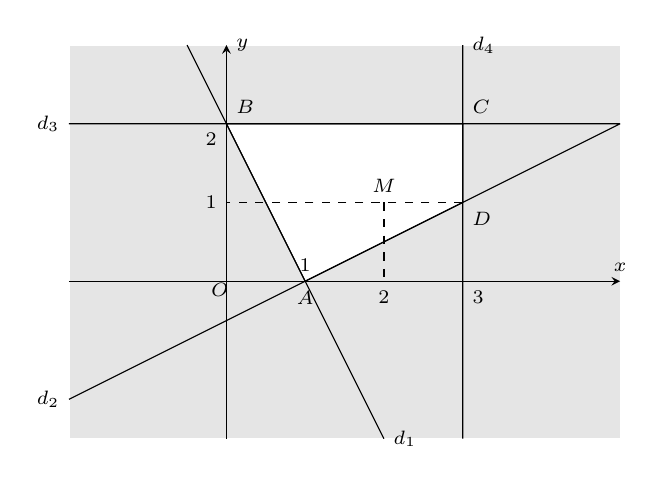
\begin{tikzpicture}[>=stealth]
				\draw[color=white,fill=black!10] (-2,-2) rectangle (5,3);
				\path (-1/2,3) coordinate (A1);
				\path (2,-2) coordinate (B1);
				\path (-2,-3/2) coordinate (A2);
				\path (5,2) coordinate (B2);
				\path (-2,2) coordinate (A3);
				\path (5,2) coordinate (B3);
				\path (3,-2) coordinate (A4);
				\path (3,3) coordinate (B4);
				\path (intersection of A1--B1 and A2--B2) coordinate (A);
				\path (intersection of A1--B1 and A3--B3) coordinate (B);
				\path (intersection of A3--B3 and A4--B4) coordinate (C);
				\path (intersection of A2--B2 and A4--B4) coordinate (D);
				\draw[fill=white] (A) -- (B) -- (C) -- (D) -- cycle;
				\draw[->] (0,-2) -- (0,3) node[right]{\scriptsize $y$};
				\draw[->] (-2,0) -- (5,0) node[above]{\scriptsize $x$};
				\draw (0.15,0.1) node[below left]{\scriptsize $O$};
				\draw (A1) -- (B1) node[right]{\scriptsize $d_1$} (A2)node[left]{\scriptsize $d_2$} -- (B2) (A3)node[left]{\scriptsize $d_3$} -- (B3) (A4) -- (B4) node[right]{\scriptsize $d_4$};
				\draw[dashed] (A) node[above]{\scriptsize $1$} (A) node[below]{\scriptsize $A$} (B) node[below left]{\scriptsize $2$} (B) node[above right]{\scriptsize $B$} (C) node[above right]{\scriptsize $C$} (C|- 0,0) node[below right]{\scriptsize $3$} (D) node[below right]{\scriptsize $D$} -- (D-| 0,0) node[left]{\scriptsize $1$} (2,1) node[above]{\scriptsize $M$} -- (2,0)node[below]{\scriptsize $2$};
			\end{tikzpicture}
		}
	}
\end{bt}

\begin{bt}%[Lâm Hữu Phước]%[0D4B4]
	Biểu diễn hình học tập nghiệm của hệ bất phương trình
	$\left\{\begin{aligned}
		x+2y &\geq 1\\
		3x-y & \leq 2 \\
	\end{aligned}\right.$.
\end{bt}
\begin{bt}%[Lâm Hữu Phước]%[0D4B4]
	Biểu diễn hình học tập nghiệm của hệ bất phương trình
	$\left\{\begin{aligned}
		x-2y &< 1\\
		x+3y &>-2 \\
		-x+y &<2
	\end{aligned}\right.$.
\end{bt}
\begin{bt}%[Lâm Hữu Phước]%[0D4B4]
	Biểu diễn hình học tập nghiệm của hệ bất phương trình
	$\left\{\begin{aligned}
		3x+y & \leq 5\\
		x+y & \leq 4 \\
		x &\geq 0\\
		y &\geq 0
	\end{aligned}\right.$.
\end{bt}

\begin{bt}
	Một hộ nông dân định trồng đậu và cà trên diện tích $8$ ha. Nếu trồng đậu thì cần $20$ công và thu $3000000$ đồng trên diện tích mỗi ha, nếu trồng cà thì cần $30$ công và thu $4000000$ đồng trên diện tích mỗi ha. Hỏi cần trồng mỗi loại cây trên với diện tích là bao nhiêu để thu được nhiều tiền nhất biết rằng tổng số công không quá $180$?
	\loigiai{
		Gọi số ha đậu và cà mà hộ nông dân này trồng lần lượt là $x$ và $y (x,y\ge 0).$\\
		Lợi nhuận thu được là $f(x;y)=3000000x+4000000y$ (đồng).\\
		Tổng số công dùng để trông $x$ ha đậu và $y$ ha cà là $20x+30y.$\\
		Ta có hệ bất phương trình sau $\heva{&x+y\le 8\\&20x+30y\le 180\\&x, y\ge 0}\Leftrightarrow \heva{&x+y\le 8\\&2x+3y\le 18\\&x, y\ge 0}.$\\
		Bài toán trở thành tìm giá trị lớn nhất của hàm số $f(x;y)$ trên miền nghiệm của hệ bất phương trình $(*)$. Miền nghiệm của hệ bất phương trình $(*)$ là tứ giác $OABC$ (kể cả biên).\\
		Hàm số $f(x;y)$ sẽ đạt giá trị lớn nhất khi $(x;y)$ là tọa độ của một trong các đỉnh $O(0;0)$,  $ A(8;0)$,  $ B(6;2)$,  $ C(0;6)$.\\
		Ta có: $f(0;0)=0, f(8;0)=24000000, f(6;2)=26000000, f(0;6)=2400000.$\\
		Suy ra $f(x;y)$ lớn nhất khi $(x;y)=(6;2)$ tức là hộ nông dân này cần phải tròng $6$ ha đậu và $2$ ha cà thì sẽ thu về lợi nhuận lớn nhất. 
		\begin{center}
			\begin{tikzpicture}[line width=1pt,>=stealth,x=1cm,y=1cm,scale=0.5]
				\draw[->] (-1,0)--(10.2,0)
				node[below]{\footnotesize $ x $};
				\draw[->] (0,-1)--(0,10.2)
				node[right]{\footnotesize $ y $};
				\draw (0,0) node[below left]{\footnotesize $O$};
				\clip (-1,-1) rectangle (10,10);
				\draw[smooth,domain=-1:10] plot (\x,{-\x+8});
				\draw[smooth,domain=-1:10] plot (\x,{-0.67*\x+6});
				%\draw[-] (4,-1) -- (4,10);
				\fill[pattern=north west lines]
				(-6,10)--(10,10)--(10,-0.6)--cycle;
				\fill[pattern=north west lines]
				(-1,0)--(10,0)--(10,-1)--(-1,-1)--cycle;
				\fill[pattern=north west lines]
				(-1,-1)--(-1,10)--(0,10)--(0,-1)--cycle;
				\fill[pattern=north west lines]
				(-2,10)--(10,10)--(10,-2)--cycle;
				\draw (8,0) node[above]{\footnotesize$A$};
				\draw (8,0) node[below left]{\footnotesize$8$};
				\draw (6,2) node[right]{\footnotesize$B$};
				\draw (6,0) node[below]{\footnotesize$6$};
				\draw[dashed] (0,2)--(6,2);
				\draw (0,2) node[left]{\footnotesize$2$};
				\draw[dashed] (6,0)--(6,2);
				\draw (0,6) node[right]{\footnotesize $C$};
				\draw (0,6) node[left]{\footnotesize $6$};
			\end{tikzpicture}
		\end{center}
	}
\end{bt}

\begin{bt}
	Một gia đình định trồng cà phê và ca cao trên diện tích $ 10 $ ha. Nếu trồng cà phê thì cần $ 20 $ công và thu về $ 10.000.000 $ đồng trên diện tích mỗi ha, nếu trồng cà thì cần $ 30 $ công và thu $ 12.000.000 $
	đồng trên diện tích mỗi ha. Hỏi cần trồng mỗi loại cây trên với diện tích là bao nhiêu để thu được
	nhiều tiền nhất. Biết rằng cà phê do các thành viên trong gia đình tự chăm sóc và số công không
	vượt quá $ 80 $, còn ca cao gia đình thuê người làm với giá $  100.000 $ đồng cho mỗi công?
	\loigiai{
		Gọi $ x $ và $ y $ lần lượt là số ha cà phê và ca cao mà hộ nông dân này trồng $ (x, y\ge 0). $\\
		Số tiền cần bỏ ra để thuê người trồng ca cao là $ 30y . 100000=3000000 y $ (trồng).\\
		Lợi nhuận thu được là $ f(x;y)=1000000x+12000000-3000000y$ \\
		$\Rightarrow f(x;y)=10000000x+9000000y $ (đồng).\\
		Vì số công để trồng cà phê không vượt qua $ 80 $ nên $ 20x\le 80\Leftrightarrow x\le 4. $\\
		Ta có hệ bất phương trình sau $ \heva{&x+y\le 10\\&0\le x\le 4\\& y\ge 0} (*). $\\
		Ta cần tìm giá trị lớn nhất của $ f(x;y) $ trên miền nghiệm của hệ $ (*). $\\
		Miền nghiệm của hệ $  (*) $ là tứ giác $ OABC $ (kể cả biên). Hàm số $ f(x;y) $ sẽ đạt giá trị lớn nhất khi $ (x;y) $ là toạ độ của một trong các đỉnh $ O(0;0) $, $ A(4;0) $, $ B(4;6) $, $ C(0;10) $.
		Suy ra $ f(x;y) $ lớn nhất khi $ (x;y)=(4;6) $. Như vậy cần phải trồng $  4 $ ha cà phê và $ 6 $ ha ca cao để thu
		về lợi nhuận lớn nhất
		\begin{center}
			\begin{tikzpicture}[line width=1pt,>=stealth,x=1cm,y=1cm,scale=0.6]
				\pgfresetboundingbox
				\draw[->] (-1,0)--(5.2,0)
				node[below]{\footnotesize $ x $};
				\draw[->] (0,-1)--(0,11.2)
				node[right]{\footnotesize $ y $};
				\draw (0,0) node[below left]{\footnotesize $ O$};
				\clip (-1,-1) rectangle (5,11);
				\draw[smooth,domain=-1:11] plot (\x,{-\x+10});
				\draw[-] (4,-1) -- (4,11);
				\fill[pattern=north west lines]
				(-1,11)--(0,11)--(0,-1)--(-1,-1)--cycle;
				\fill[pattern=north west lines]
				(-1,0)--(11,0)--(11,-1)--(-1,-1)--cycle;
				\fill[pattern=north west lines]
				(4,-1)--(4,11)--(11,11)--(11,-1)--cycle;
				\fill[pattern=north west lines]
				(-1,11)--(11,11)--(11,-1)--cycle;
				\draw (4,0) node[above left]{\footnotesize$A$};
				\draw (4,0) node[below left]{\footnotesize$4$};
				\draw (4,6) node[below left]{\footnotesize $B$};
				\draw (-0.2,9.6) node[below right]{\footnotesize $C$};
				\draw (0,10) node[right]{\footnotesize $10$};
			\end{tikzpicture}
		\end{center}
	}
\end{bt}
\begin{bt}%[0D4G4-4]
	Quảng cáo sản phẩm trên truyền hình là một hoạt động quan trọng trong kinh doanh của các doanh nghiệp.\\
	Theo Thông báo số $10/2019$, giá quảng cáo trên VTV1 là $30$ triệu đồng cho $15$ giây/$1$ lần quảng cáo vào khoảng $20$h$30$; là $6$ triệu đồng cho $15$ giây/$1$ lần quảng cáo vào khung giờ $16$h$00-17$h$00$.\\
	Một công ty dự định chi không quá $900$ triệu đồng để quảng cáo trên VTV1 với yêu cầu quảng cáo về số lần phát như sau: ít nhất $10$ lần quảng cáo vào khoảng
	$20$h$30$ và không quá $50$ lần quảng cáo vào khung giờ $16$h$00-17$h$00$. Hỏi công ty có thể phát tối đa bao nhiêu lần quảng cáo?
	\loigiai{
		Gọi $x, \,y$ lần lượt là số lần phát quảng cáo vào khoảng $20$h$30$  và vào khung giờ $16$h$00-17$h$00$. Theo giả thiết, ta có: $x \in \mathbb{N},\, y \in \mathbb{N},\, x \geq 10,0 \leq y \leq 50$.\\
		Tổng số lần phát quảng cáo là $T=x+y$.\\
		Số tiền công ty cần chi là $30 x+6 y$ (triệu đồng).\\
		Do công ty dự định chi không quá $900$ triệu đồng nên $30 x+6 y \leq 900$ hay $5 x+y \leq 150$.\\
		Ta có hệ bất phương trình: $\heva{5 x+y \leq 150 \\ x \geq 10 \\ 0 \leq y \leq 50.} $ \hfill(I)	
		Bài toán đưa về tìm $x, y$ là nghiệm của hệ bất phương trình (I) sao cho $T=x+y$ có giá trị lớn nhất.\\
		Trước hết, ta xác định miền nghiệm của hệ bất phương trình (I).\\
		Miền nghiệm của hệ bất phương trình (I) là miền tứ giác $A B C D$ với $A(30 ; 0), B(20 ; 50)$, $C(10 ; 50), D(10 ; 0)$ (Hình vẽ).
		\immini{
			Người ta chứng minh được: Biểu thức $T=x+y$ đạt được giá trị lớn nhất tại một trong các đỉnh của tứ giác $A B C D$.
			Tính giá trị của biểu thức $T=x+y$ tại cặp số $(x ; y)$ là toạ độ các đỉnh của tứ giác $A B C D$ rồi so sánh các giá trị đó. Ta được $T$ đạt giá trị lớn nhất khi $x=20, y=50$ ứng với tọa độ đỉnh $B$.\\
			Vậy để phát được số lần quảng cáo nhiều nhất thì số lần phát quảng cáo vào khoảng $20$h$30$  và vào khung giờ $16$h$00-17$h$00$  lần lượt là $20$ và $50$ lần.
		}{\begin{tikzpicture}[scale=0.07,line join=round, line cap=round,>=stealth,thick]
				\tikzset{label style/.style={font=\footnotesize}}
				\begin{scope}
					
					\clip (-20,-20) rectangle (60,60);
					\fill[pattern=crosshatch dots] (-21,255)--(61,255)--(61,-155)--cycle;
					\fill[pattern=crosshatch dots] (10,-20)--(-20,-20)--(-20,60)--(10,60)--cycle;
					\fill[pattern=crosshatch dots] (-20,0)--(-20,-20)--(60,-20)--(60,0)--cycle;
					\fill[pattern=crosshatch dots] (-20,50)--(-20,60)--(60,60)--(60,50)--cycle;
					\draw (18,60)--(34,-20) ;
					\draw (10,-20)--(10,60) ;
					\draw (-20,50)--(60,50) ;
				\end{scope}
				\draw[->] (-20,0)--(60,0) node[below]{$x$};
				\draw[->] (0,-20)--(0,60) node[left]{$y$};
				\draw (0,0) node[below left]{$O$};
				\path (10,50) coordinate(C) (10,0) coordinate(D) (30,0) coordinate(A) (20,50) coordinate(B);
				\foreach \i in {A,B,C,D} \fill (\i) circle(20pt) ($(\i)+(55:5)$)node{$\i$};
				\foreach \x in {10,20,30}
				\draw[thin] (\x,1pt)--(\x,-1pt) node [below right] {$\x$};
				\foreach \y in {50}
				\draw[thin] (1pt,\y)--(-1pt,\y) node [below left] {$\y$};
		\end{tikzpicture}}
	}
\end{bt}

\begin{bt}%[BG10-2022]%[Toanvo]%[0D4G4-4]
	Một gia đình cần ít nhất $900$ đơn vị protein và $400$ đơn vị lipit trong thức ăn mỗi ngày. Mỗi kg thịt bò chứa $800$ đơn vị protein và $200$ đơn vị lipit. Mỗi kg thịt lợn chứa $600$ đơn vị protein và $400$ đơn vị lipit. Biết rằng mỗi ngày gia đình này chỉ mua tối đa $1{,}5$ kg thịt bò và $1$ kg thịt lợn, giá tiền $1$ kg thịt bò là $200$ nghìn đồng, $1$ kg thịt lợn là $100$ nghìn đồng. Hỏi gia đình đó phải mua bao nhiêu kg thịt mỗi loại để số tiền bỏ ra là ít nhất.
	\loigiai{
		Gọi số kg thịt bò cần mua là $x$ (kg); số kg thịt lợn cần mua là $y$ (kg). Điều kiện: $0 \leq x \leq 1{,}5, 0 \leq y \leq 1$.\\
		Khi đó số đơn vị protein là $800x+600y$.\\
		Số đơn vị lipit là $200x+400y$.\\
		Ta có hệ bất phương trình $$\heva{&0\leq x\leq 1{,}5\\&0\leq y\leq 1\\&800x+600y\geq 900\\&200x+400y\geq200}\Leftrightarrow\heva{&0\leq x\leq 1{,}5\\&0\leq y\leq 1\\&8x+6y\geq9\\&x+2y\geq2.}$$	
		Vẽ các đường thẳng $(d_1)\colon x=1{,}5$, $(d_2)\colon y=1$, $(d_3)\colon 8x+6y=9$, $(d_4)\colon x+2y=2$. Ta được miền nghiệm của hệ bất phương trình là phần tô đậm trong hình vẽ.
		\begin{center}
			\begin{tikzpicture}[line join = round, line cap = round, >=stealth, font=\footnotesize, scale=1.2]
				\tikzset{label style/.style={font=\footnotesize}}
				\def \xmin{-3.5}
				\def \xmax{5.5}
				\def \ymin{-1.5}
				\def \ymax{6}
				\tkzDefPoints{0.375/1/A, 1.5/1/B, 1.5/0.25/C, 0.6/0.7/D}
				\draw[gray!20](\xmin,\ymin) grid (\xmax,\ymax);
				\draw [->](\xmin,0)--(0,0)node[below left]{$O$}--(\xmax,0)node[above]{$x$};
				\draw [->](0,\ymin)--(0,\ymax)node[right]{$y$};
				\foreach \x in {-3,-2,-1,1,2,3,4,5} \draw[shift={(\x,0)}] (0pt,2pt)--(0pt,-2pt) node[below]{$\x$};
				\foreach \y in {-1,2,3,4,5} \draw [shift={(0,\y)}] (2pt,0pt)--(-2pt,0pt) node[left]{$\y$};
				\draw [shift={(0,1)}] (2pt,0pt)--(-2pt,0pt) node[below left]{$1$};
				\tkzDrawLine[add=6 and 2](B,C)
				%\tkzDrawLine[add=0.5 and 0.5](B,C A,B A,D D,C)
				\tkzDrawLine[add=3 and 3](A,B)
				\tkzDrawLine[add=12 and 6](A,D)
				\tkzDrawLines[add=4 and 2](D,C)
				\tkzDrawPoints[fill=black](A,B,C,D)
				\tkzLabelPoints[above right](A,B,C)
				\tkzLabelPoints[below](D)
				\tkzFillPolygon[color=cyan,fill opacity=.5](A,B,C,D)
				\tkzLabelLine[pos=7,right](C,B){$(d_1)$}
				\tkzLabelLine[pos=3.5,above right](A,B){$(d_2)$}
				\tkzLabelLine[pos=12,above right](D,A){$(d_3)$}
				\tkzLabelLine[pos=5,above right](C,D){$(d_4)$}
			\end{tikzpicture}
		\end{center}
		Ta có 
		{\allowdisplaybreaks
			\begin{eqnarray*}
				&&A\left(\dfrac{3}{8};1\right)=(d_3) \cap (d_2), B(1{,}5;1)=(d_1) \cap (d_2),\\
				&&C(1{,}5;0{,}25)=(d_1) \cap (d_4), D\left(\dfrac{3}{5};\dfrac{7}{10}\right)=(d_3) \cap (d_4).
			\end{eqnarray*}
		}
		Số tiền bỏ ra là $f(x,y)=200x+100y$ (nghìn đồng).
		\begin{center}
			\renewcommand\arraystretch{1.6}
			\renewcommand{\tabcolsep}{6mm}
			\begin{tabular}{|c|c|c|c|c|}
				\hline 
				$M(x;y)$& $A$ & $B$ & $C$ & $D$ \\ 
				\hline 
				$f(x,y)=200x+100y$& $175$ & $400$ & $325$ & $190$ \\ 
				\hline 
			\end{tabular} 
		\end{center}
		Do đó $f(x,y)$ đạt giá trị nhỏ nhất tại $A\left(\dfrac{3}{8};1\right)$.\\
		Vậy để số tiền bỏ ra nhỏ nhất thì cần mua $\dfrac{3}{8}$ kg thịt bò và $1$ kg thịt lợn.
	}
\end{bt}